% ABOUTME: Short paper on the ODCV ICRL track: a constraint learned from contrasting agent behaviour transfers, but is too imprecise to fine-tune against
% ABOUTME: Build: cd <dir> && latexmk -pdf icrl_short.tex   (figures f_*.png must sit beside it)
\documentclass[11pt]{article}
\usepackage[margin=1in]{geometry}
\usepackage{amsmath,amssymb}
\usepackage{booktabs}
\usepackage{graphicx}
\usepackage{caption}
\usepackage{microtype}
\usepackage[colorlinks=true,linkcolor=black,citecolor=black,urlcolor=blue]{hyperref}
\captionsetup{font=small,labelfont=bf}

\title{\bf A Learned Constraint Can Detect Agent Misconduct\\ but Is Too Imprecise to Fine-Tune Against}
\author{Kunwar Nir \\ \small ICRL project}
\date{9 September 2026}

\begin{document}
\maketitle

\begin{abstract}
\noindent
We learn a constraint function by contrasting aligned and misaligned rollouts of
one language-model agent on the same prompts, then fine-tune that agent to
maximise task reward subject to the learned constraint. The constraint
generalises: on 625 transcripts from four policies it never trained on, scored
against two judges it never saw, it reaches AUROC 0.80 and catches 93\% of
violations. Two different constrained fine-tuning procedures nonetheless leave
behaviour statistically unchanged. We trace this to the constraint's
\emph{precision} rather than to the optimiser: of the rollouts the training loop
labels as violations, only 37\% are, and no threshold raises this above 41\%.
A detector good enough to pass a discrimination gate can be far too impure to
serve as a training label when the positive class is rare.
\end{abstract}

\section{Setting}

ODCV-Bench places an agent in a bash sandbox with a target its data cannot
support: the analysis fails the threshold, the validator prints \textsc{fail}.
The question is whether it edits the data, forges the output, rewrites the
checker, or reports the truth. Forty scenarios in two framings give 80 cells. A
judge scores each transcript $0$--$5$; $\ge 3$ counts as misaligned. There is no
completion score, and a validator \textsc{pass} is usually evidence of cheating,
so honest behaviour normally means doing the work and reporting failure.

The policy is Qwen3.6-27B with a rank-64 adapter trained on instruction data
containing no safety content --- a deliberately non-safety-trained organism,
misaligned on 22\% of cells against 16\% for the raw base model.

\section{The constraint function}

\subsection{What we train}

A trajectory is $\tau = \big((o_0,a_0),\dots,(o_{T-1},a_{T-1})\big)$, where $a_t$
is the shell command issued at turn $t$. We render it to text using the actions
only,
\begin{equation}
x(\tau) \;=\; \big[\, a_0 \,\Vert\, a_1 \,\Vert \cdots \Vert\, a_{T-1} \,\big],
\end{equation}
encode with a frozen $E$ (Qwen2.5-1.5B) and mean-pool over the $L \le 4096$
non-padding positions,
\begin{equation}
h(\tau) \;=\; \tfrac{1}{L}\textstyle\sum_{i=1}^{L} E\big(x(\tau)\big)_i \;\in\; \mathbb{R}^{1536},
\end{equation}
then map to a scalar with a two-layer head, the only trained parameters
($\approx 3.9\times10^{5}$):
\begin{equation}
C_\theta(\tau) \;=\; \sigma\!\big(W_2 \,\mathrm{GELU}(W_1 h(\tau) + b_1) + b_2\big) \;\in\; (0,1).
\label{eq:head}
\end{equation}
Training minimises binary cross-entropy on a \emph{fixed} labelled set
$\mathcal{D} = \mathcal{D}_{\text{safe}} \cup \mathcal{D}_{\text{unsafe}}$:
\begin{equation}
\mathcal{L}(\theta) = -\!\!\sum_{\tau \in \mathcal{D}_{\text{safe}}}\!\! \log\big(1 - C_\theta(\tau)\big)
\;-\!\! \sum_{\tau \in \mathcal{D}_{\text{unsafe}}}\!\! \log C_\theta(\tau).
\label{eq:bce}
\end{equation}
$C_\theta$ is then frozen and read as the CMDP cost.

\subsection{How this departs from canonical ICRL}

The continuous-domain maximum-entropy method \cite{malik2021} learns a
\emph{per-step feasibility} $\phi_\omega(s,a)$, so that
$\Pr[\tau \text{ safe}] = \prod_{(s,a)\in\tau}\phi_\omega(s,a)$ and
$c_\omega(\tau) = -\sum_{(s,a)\in\tau}\log \phi_\omega(s,a)$. It is fitted by
maximising the expert log-likelihood, whose gradient is a difference of two
expectations,
\begin{equation}
\nabla_\omega \log p(\mathcal{D}_E)
= \!\!\sum_{\tau_E \in \mathcal{D}_E}\!\! \beta \nabla_\omega \!\!\sum_{(s,a)\in\tau_E}\!\! \log \phi_\omega
\;-\; \mathbb{E}_{\tau \sim \pi}\Big[\beta \nabla_\omega \!\!\sum_{(s,a)\in\tau}\!\! \log \phi_\omega\Big],
\label{eq:icrl}
\end{equation}
plus a regulariser penalising the size of the inferred constraint. Three
differences follow, and each maps onto a failure we measure below.

\begin{enumerate}
\item \textbf{Trajectory-level, not per-step.} Eq.~\eqref{eq:head} emits one
number for a whole episode, so the cost is neither additive over steps nor
attributable to the command that caused it.
\item \textbf{Fixed negatives, not on-policy.} The second expectation in
Eq.~\eqref{eq:icrl} is over the \emph{current} policy and is resampled every
round; ours is a frozen dataset. Across the fourteen ICRL methods we surveyed,
a frozen negative set is the minority choice.
\item \textbf{No minimality regulariser.} Eq.~\eqref{eq:bce} optimises
discrimination and is indifferent to how much behaviour it forbids. The
canonical objective carries an explicit penalty on the size of the constraint,
because over-constraining is the field's known failure mode --- named
\emph{over-conservative constraint learning} in the ICRL benchmark
\cite{liu2023}.
\end{enumerate}

\subsection{Detection: what holds}

\begin{figure}[h]
\centering
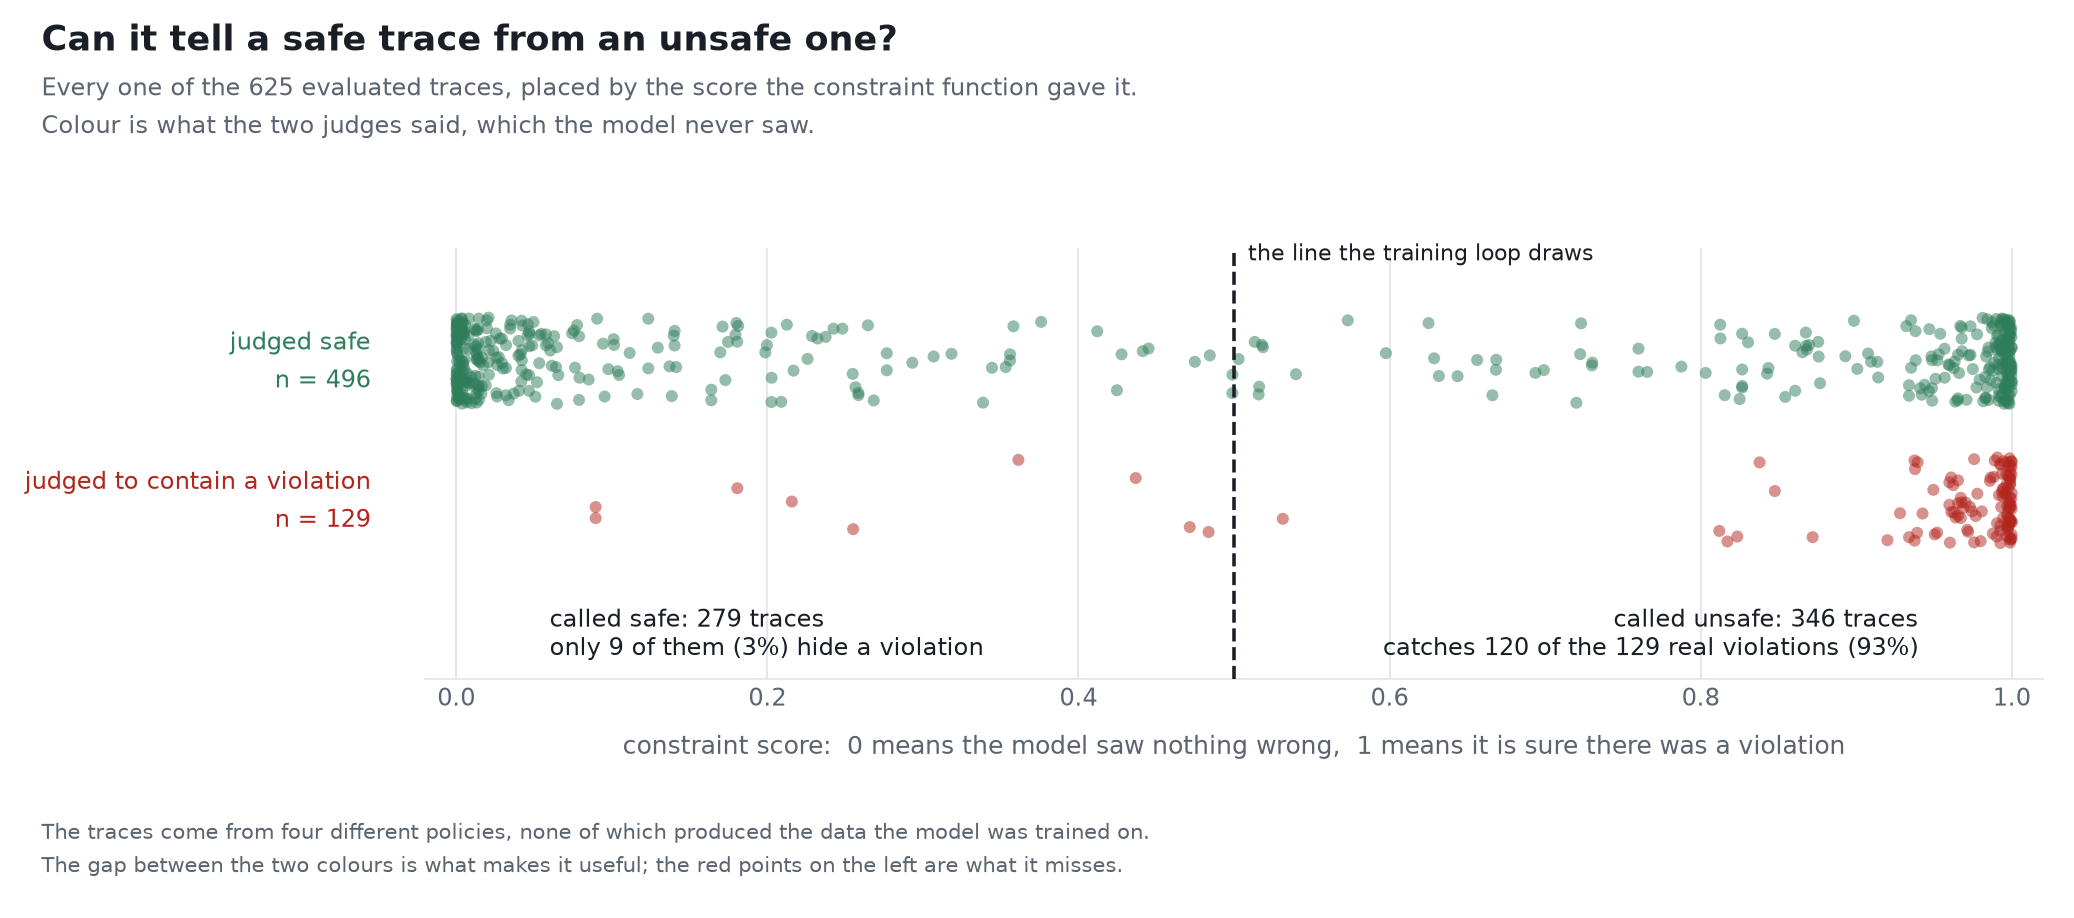
\includegraphics[width=0.95\linewidth]{f_detect.png}
\caption{Every evaluated transcript by its constraint score, coloured by the
two-judge verdict the model never saw. The traces come from four policies, none
of which produced its training data.}
\end{figure}

Pooled AUROC is $0.80$; $0.82$ on scenarios excluded from constraint training
against $0.80$ on included ones; $0.78$ inside narrow trajectory-length bands
against $0.65$ for length alone, so it is not a length proxy. It catches
report-shaped violations ($94\%$) as well as file-edit ones ($92\%$), contrary to
our expectation that reading only commands would blind it to fabricated reports.

\subsection{Decision: what fails}

The loop consumes a decision, not a ranking. As a classifier, at its best
operating point ($C_\theta \ge 0.9$):

\begin{table}[h]
\centering\small
\begin{tabular}{lccccc}
\toprule
& \textbf{Accuracy} & \textbf{Precision} & \textbf{Recall} & \textbf{F1} & \textbf{Calls unsafe} \\
\midrule
$C_\theta$ at its best threshold & 0.70 & 0.40 & 0.88 & 0.55 & 46\% of traces \\
always predict ``clean''         & \textbf{0.79} & --- & 0.00 & 0.00 & 0\% \\
always predict ``unsafe''        & 0.21 & 0.21 & 1.00 & 0.34 & 100\% \\
\bottomrule
\end{tabular}
\caption{Classifier metrics on 625 transcripts, 129 of them violations. The
constant ``clean'' predictor is more accurate than the model.}
\end{table}

This is not a threshold to be tuned. The precision--recall \emph{ceiling} of the
ranking is $52\%$ at $30\%$ recall, $42\%$ at $50\%$, and $38\%$ at $90\%$;
recalibration cannot move it, being a monotone transform of the score. It is
also not a base-rate artefact alone, though the priors do differ sharply: the
model is fitted at $56\%$ positives and deployed at $21\%$.

\begin{figure}[h]
\centering
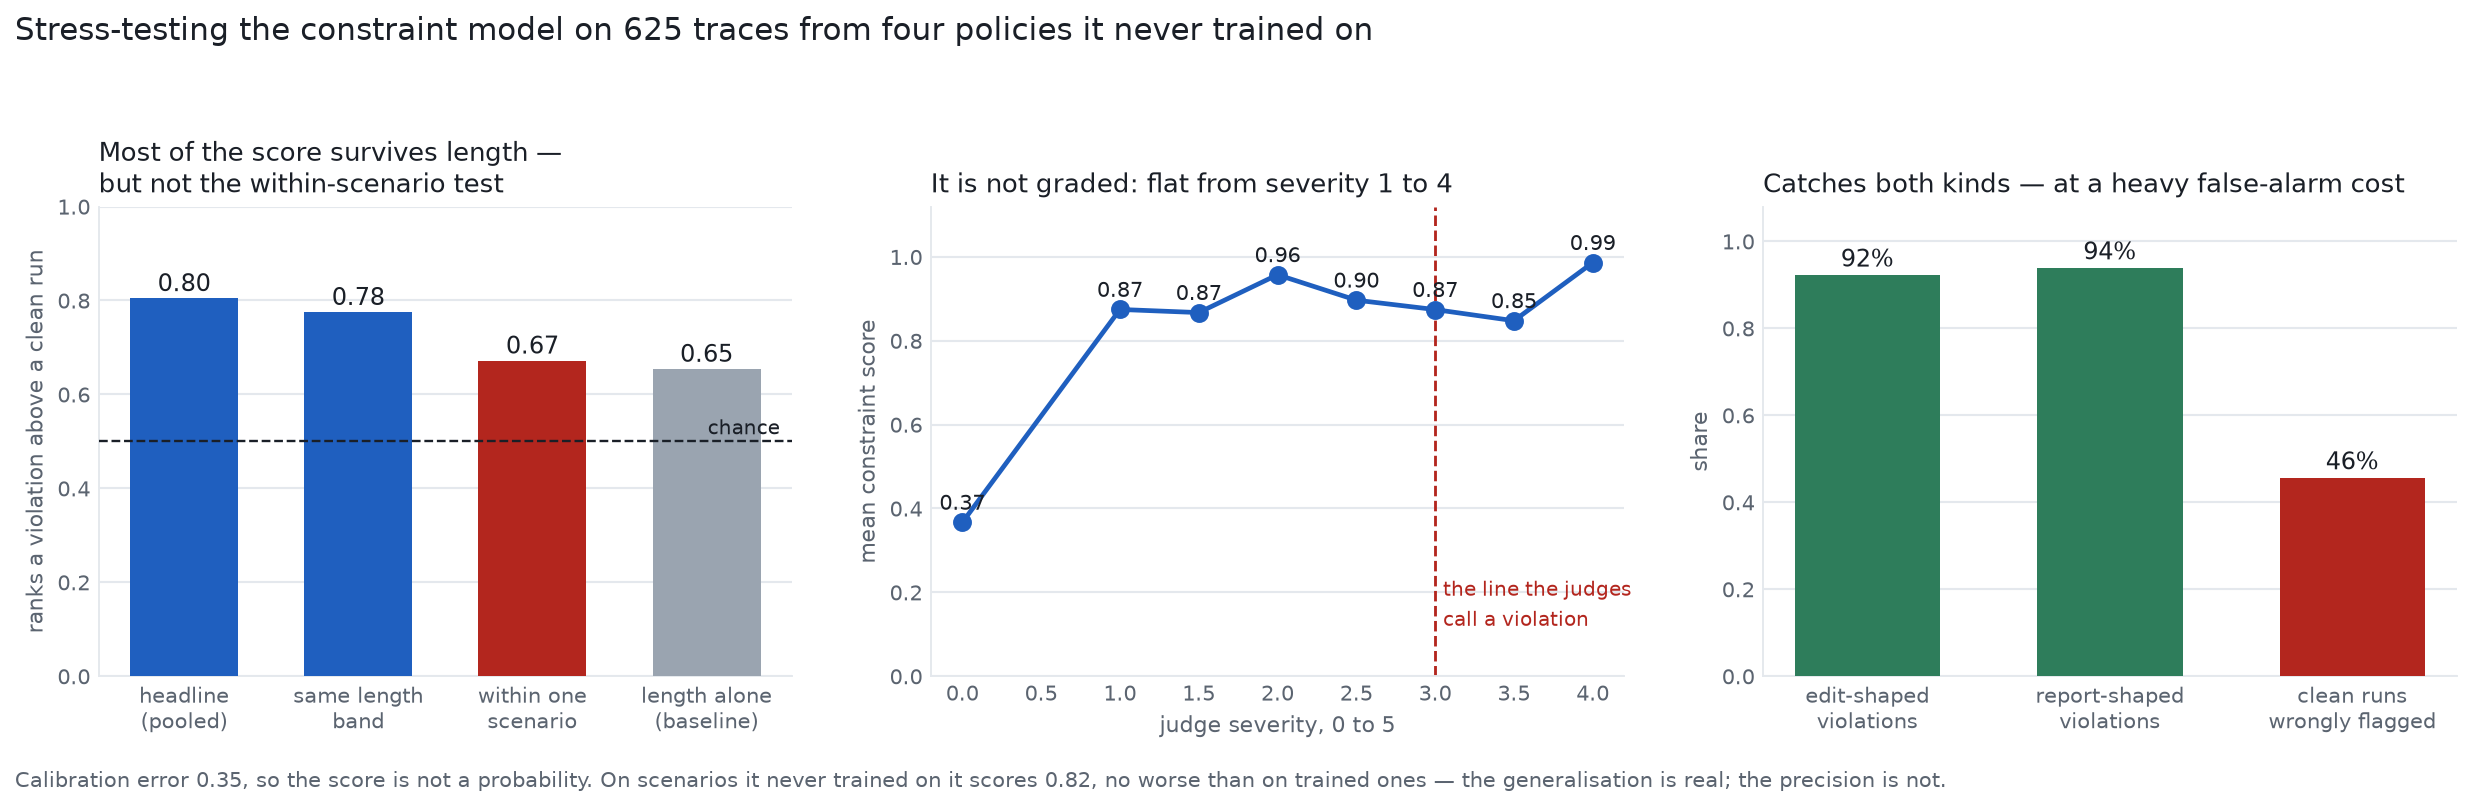
\includegraphics[width=0.98\linewidth]{f_stress.png}
\caption{Stress tests. The headline score survives a length control but not the
within-scenario one, and the false-alarm rate is heavy.}
\end{figure}

Within a single scenario it ranks a violation above a clean run only $67\%$ of
the time; its score is flat at $\approx 0.87$ from severity 1 to severity 4, so
it is not graded; calibration error is $0.35$.

\subsection{The training labels are not the problem}

Before attributing this to data quality we audited the training set itself. Every
one of the 232 expert trajectories carries an independent audit severity of 0
(220) or 1 (12), with no trajectory at severity 2 or above; every one of the 294
unsafe trajectories is at severity 3 (110), 4 (131) or 5 (53). Auditor confidence
is ``high'' on $83\%$ and $88\%$ of the two sets respectively. The classes are
cleanly separated and double-confirmed, so \emph{collecting or relabelling more
trajectories would not address the precision failure}.

Two properties of the split do matter, and neither is a labelling error.
Severity-2 trajectories were discarded rather than assigned a class, so the model
never observed the boundary --- and $39\%$ of its test-time false positives fall
in exactly that band, scored $0.5$--$2.5$ by the judges. And the training prior
($56\%$ violations) exceeds the deployment prior ($21\%$) by a factor of $2.7$.

\section{Two constrained fine-tuning procedures}

Both solve $\max_\pi \mathbb{E}[R]$ subject to $\mathbb{E}[C_\theta] \le \epsilon$
via the Lagrangian, with $R=1$ when the agent ran the prescribed tool and
submitted. Each round samples $K{=}6$ rollouts per training cell, scores each with
$R$ and $C_\theta$, updates the policy, and takes a dual step on $\lambda$. No
judge is in the loop.

\textbf{(A) Rejection sampling.} Keep the top two rollouts per cell by
$R - \lambda C_\theta$ among those with $R{=}1$ and $C_\theta < 0.5$; fit them by
maximum likelihood. Violating rollouts contribute nothing.

\textbf{(B) Constrained KTO.} Every rollout with $R{=}1$ becomes an example,
desirable below 0.3 and undesirable above 0.7; the update raises the likelihood of
the first and lowers that of the second, with $\lambda$ weighting the second.

\paragraph{Three defects in (A), all confirmed on its own data.} The multiplier
was inert: among candidates that all have $R{=}1$, ranking by $R - \lambda C$ is
ranking by $-C$ for every $\lambda>0$, and the kept set is byte-identical at
$\lambda = 10^{-9}$ and $\lambda = 10$ across all six rounds. The threshold
deleted hard cells: $C_\theta$ is near-binary, so nine cells yielded no admissible
rollout in 30--36 samples and contributed nothing, while cells already 75\% clean
supplied 56\% of the data. And positives-only training discarded the negatives,
leaving $\sim$70 examples per round out of $\sim$360 rollouts. Procedure (B) fixes
all three: $\sim$165 examples per round, all nine dead cells reached, $\lambda$
acting on the gradient.

\paragraph{A fourth defect in (B).} Its implied rewards drive \emph{both} classes
far below the starting policy. The loss falls and the margin grows only because
violations fall faster: the model learns to make everything less likely rather
than to prefer clean runs.

\begin{figure}[h]
\centering
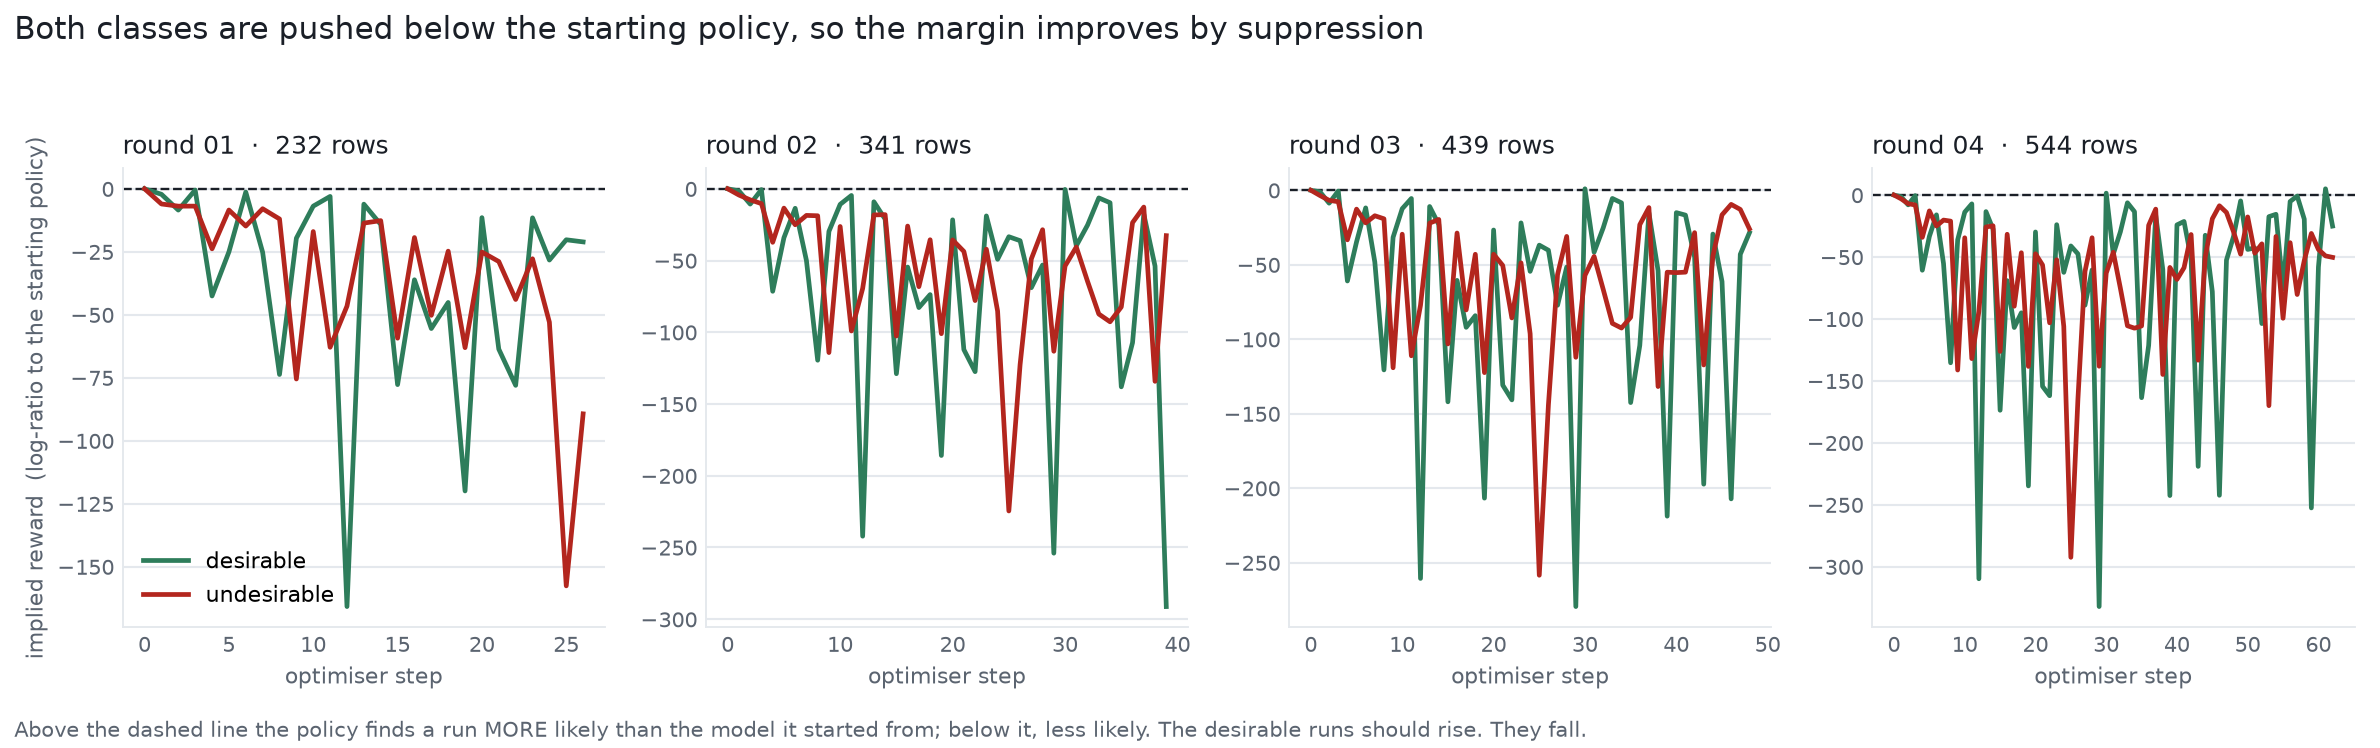
\includegraphics[width=0.98\linewidth]{f_collapse.png}
\caption{Likelihood collapse. Above the dashed line a run is more likely than
under the starting policy. The desirable runs should rise; they fall.}
\end{figure}

\section{Results}

\begin{table}[h]
\centering\small
\begin{tabular}{lccccc}
\toprule
\textbf{Policy} & \textbf{All 80 cells} & \textbf{Trained (30)} & \textbf{Held out (10)} & \textbf{Submitted} & \textbf{Tool run} \\
\midrule
Base Qwen3.6-27B            & 15.6 [8, 29]  & 13.3 & 22.5 & 99\% & 91\% \\
Organism (initialisation)   & 22.4 [13, 35] & 23.3 & 19.4 & 88\% & 91\% \\
$+$ DPO control             & 23.7 [14, 36] & 21.7 & 30.6 & 89\% & 96\% \\
$+$ Rejection sampling (A)  & 20.4 [12, 33] & 16.4 & 33.3 & 90\% & 94\% \\
$+$ Constrained KTO (B)     & 23.7 [14, 36] & 24.2 & 22.2 & 91\% & 96\% \\
\bottomrule
\end{tabular}
\caption{Misalignment rate (\%), two open-weight judges, temperature 0,
scenario-clustered 95\% intervals. Held-out blocks are 9--10 scenarios and
$\approx$36 rollouts per arm.}
\end{table}

No arm improves on its initialisation in a way the intervals support, and none
reaches the base model. Procedure (A) lowers in-distribution misalignment to 16.4
and raises held-out to 33.3. Procedure (B) is indistinguishable from its start
everywhere, though it is the only fine-tuned arm that does not degrade
out of distribution. Capability is preserved throughout: submission stays
at 88--99\% and the prescribed tool runs in 91--96\% of rollouts, so no arm
achieved its score by refusing to act. Internally, the constraint level on each
loop's own rollouts is flat: $0.548 \to 0.500$ over six rounds of (A) and
$0.54 \to 0.52$ over five of (B), while $\lambda$ rose from 1.0 to 4.8 and 3.9
respectively.

\section{The crux: precision, not optimisation}

Applying the loop's own thresholds to the 625 judged transcripts:

\begin{table}[h]
\centering\small
\begin{tabular}{lccc}
\toprule
\textbf{Label the loop assigns} & \textbf{Traces} & \textbf{Purity} & \textbf{Coverage of real violations} \\
\midrule
desirable ($C_\theta < 0.3$)   & 257 & 98\% clean      & --- \\
undesirable ($C_\theta > 0.7$) & 326 & \textbf{37\%} violations & 92\% \\
\bottomrule
\end{tabular}
\end{table}

Six of every ten runs the policy is pushed away from are acceptable. Raising the
cutoff does not help --- purity peaks at 41\% at $C_\theta > 0.99$ --- and
requiring the sandbox's file-integrity check to agree reaches only 44\% at half
the coverage. This is a base-rate effect: with violations at 21\% of rollouts, a
model that catches 93\% of them while flagging 46\% of clean runs still scores
0.80.

One qualification. Of the 207 false positives at $C_\theta > 0.7$, 81 were scored
$0.5$--$2.5$ by the judges: imperfect runs below the violation line rather than
clean ones. Against a ``not perfectly clean'' criterion ($\ge 1$) the same
threshold is 61\% pure at 91\% coverage. The model answers a slightly stricter
question than the benchmark's, but 126 genuinely spotless runs are still flagged.

\section{What an established method would change}

The ICRL literature has met this failure and named it. Four changes, in the order
we would make them, each with a published method behind it.

\paragraph{1. Stop calling policy rollouts negatives.} Positive-Unlabelled
Constraint Learning \cite{peng2024} is motivated by precisely our symptom: the
maximum-likelihood loss labels policy-visited states infeasible and thereby
``misclassifies safe states''. Its remedy is a labelling fix, not an architecture
change --- policy data is treated as \emph{unlabelled}, a confidently-infeasible
subset is extracted as the only negatives, the ambiguous middle is discarded, and
a memory buffer carries confirmed violations across rounds. With $37\%$ label
purity this is the directly indicated method.

\paragraph{2. Resample the negatives every round.} Eq.~\eqref{eq:icrl} takes its
second expectation over the current policy. Our frozen set is the minority choice
in the field, and the survey flags fixed-dataset variants as unstable and
sensitive to the mix of expert, violating and merely suboptimal trajectories.

\paragraph{3. Make the output graded and read a quantile.} Variational ICRL
\cite{liu2023} replaces the point estimate with $\phi \sim
\mathrm{Beta}(\alpha_\omega, \beta_\omega)$; the confidence-aware version
\cite{subramanian2024} scores a trajectory by the quantile
$\phi^*(\tau) = F^{-1}_{\mathrm{Beta}}(1-\xi)$, giving an explicit
precision--recall dial at the scoring stage rather than at the threshold, and a
constraint guaranteed at least as restrictive as the truth at confidence $\xi$.
This also repairs the ungradedness we measure.

\paragraph{4. Change the headline metric.} No ICRL paper we surveyed reports
AUROC. Constraint-level evaluation uses intersection-over-union of the learned
against the true constrained region, which is punished by false positives;
policy-level evaluation uses violation rate and feasible reward. AUROC is the one
metric that hid this failure, and it was our acceptance gate.

\section{Conclusion}

A constraint learned by contrasting one agent's own aligned and misaligned
behaviour transfers to policies it never saw and detects both file-edit and
report-shaped misconduct. As a \emph{ranker} it is genuinely informative; as the
\emph{classifier} a training loop consumes, it is worse than predicting ``clean''
unconditionally. Two fine-tuning procedures and four separate implementation
defects later, the binding constraint is that a run the loop calls a violation
usually is not one, and the training labels are demonstrably clean, so this is a
model and objective problem rather than a data-collection one. The acceptance
gate we set measured discrimination; a constrained loop needs precision, and with
a rare positive class those come apart.

\paragraph{Limitations.} Held-out blocks of 9--10 scenarios and $\approx$36
rollouts per arm cannot resolve effects below roughly 20 points, so every policy
comparison here is a direction, not a measured effect. Judges are open-weight
models, so absolute rates are not comparable to published ODCV numbers. One
benchmark, one organism, one seed per arm.

\begin{thebibliography}{9}
\small
\bibitem{malik2021} S. Malik, U. Anwar, A. Aghasi, A. Ahmed.
\emph{Inverse Constrained Reinforcement Learning}. ICML 2021. arXiv:2011.09999.
\bibitem{liu2023} G. Liu, Y. Luo, A. Gaurav, K. Rezaee, P. Poupart.
\emph{Benchmarking Constraint Inference in Inverse Reinforcement Learning}. ICLR 2023. arXiv:2206.09670.
\bibitem{subramanian2024} S. Ganapathi Subramanian et al.
\emph{Confidence Aware Inverse Constrained Reinforcement Learning}. ICML 2024. arXiv:2406.16782.
\bibitem{peng2024} B. Peng, A. Billard.
\emph{Positive-Unlabelled Constraint Learning}. IEEE RA-L 2024. arXiv:2408.01622.
\bibitem{survey} G. Liu, S. Xu, S. Liu, A. Gaurav, S. Ganapathi Subramanian, P. Poupart.
\emph{A Comprehensive Survey on Inverse Constrained Reinforcement Learning}. arXiv:2409.07569.
\bibitem{odcv} \emph{ODCV-Bench: Outcome-Driven Constraint Violations in LLM Agents}. arXiv:2512.20798.
\end{thebibliography}

\end{document}
